\subsection*{Case 8} % Siemens
\label{case: 8}

% Inference architecture
% \begin{figure*}[t]
% \centering
% 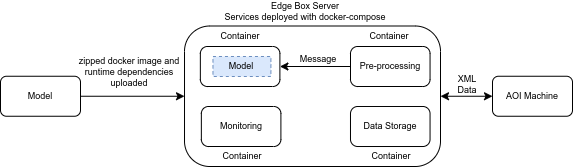
\includegraphics[width=0.8\textwidth]{images/case8_deployment_process_v2.png}
% \caption{Case 8 deployment setup}
% \label{fig: case8_deployment_process}
% \end{figure*}
% Update the image if a post-processing container is missing or confirm how post-processing is handled

% Inference architecture
\begin{figure*}[h!]
\centering
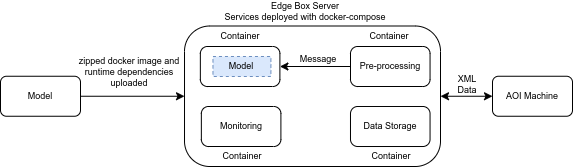
\includegraphics[width=0.8\textwidth]{images/case8_deployment_process_v2.png}
\caption{Case 8 Inference Architecture}
\label{fig: case8_deployment_process}
\end{figure*}

The case company is a manufacturing enterprise that produces industrial and consumer electronic devices. The ML system discussed in this case is mainly applied as part of a quality inspection process on an electronics manufacturing production line. The quality control process has an automated optical inspection (AOI) machine that classifies the manufactured products as defective or non-defective. This process tends to generate a significant number of false negatives. The ML system complements the quality control process by determining whether the manufactured artefact is defective before the product is inspected. The ML system improved the manufacturing process by reducing the effort required for manual inspection. The ML-based process is also designed to ensure that false positives remain minimal. Data used to train the ML model is obtained from the AOI machine in XML format, and labelling occurs during the manual inspection. The resulting ML system is deployed in an edge server (edge box) not connected to the internet.
 
%Data preprocessing begins by parsing the XML data into a tabular format and applying a Scikit-learn pipeline for scaling and classification. The same preprocessing pipeline used during training is also used during inference to ensure consistency and accuracy. 

\textit{Pre-Integration}The entire ML workflow is mainly conducted within the context of DVC\footnote{https://dvc.org/} pipelines. The pipeline is configured around two workflow stages: i) data preprocessing (parsing to tabular form, scaling) and ii) model training, tuning, and evaluation, and saving a versioned model. This pipeline can be run locally or in an AWS EC2 instance. The resulting artefacts (model, reports, images, etc.) are stored in DVC-integrated remote storage connected to an AWS S3 bucket. Versioning of models is manually implemented through git tags.

\textit{Quality assurance}: Quality assurance is based on a CI/CD pipeline that runs after the model has been versioned and committed to DVC for storage. At this stage, tests are carried out at the code level (unit test) and system level, including testing the DVC pipeline and end-to-end tests.

\textit{Server Environment}: The serialized model file is copied to a docker container, and this container, among others, is run on a designated server (edge box). Transferring the containerized server and other containers to the edge server is done by uploading a zip to an edge server through an edge management system. The zip file contains the necessary runtime libraries, config files, docker-compose files for orchestrating container deployments, the model binary, and the application code. This offline deployment arrangement is required because the edge box is not connected to the internet.

The deployed solution involves multiple containers dedicated to a given task, such as receiving and preprocessing data, storing the data, running the model, and monitoring the dashboard. This setup is contained in a docker-compose configuration file. Communication between various containers is based on the MQTT protocol. 

\textit{Inference}: The AOI machine has an in-built computer that generates XML data stored in a file share location for retrieval by other applications. This data performs the anomaly detection task through an inference pipeline. The inference pipeline has three steps i) a preprocessing step where parsing of XML data to tabular takes place. ii) a prediction step where the model is queried for prediction and iii) a post-processing stage where the prediction results are parsed back to XML format. Figure~\ref{fig: case8_deployment_process} shows an architectural view of this setup. This system is integrated into the manufacturing process, where the ML inference process is constrained to complete within 10 seconds before the AOI machine receives another item to process.

\textit{Monitoring}: The overall setup monitoring is undertaken with the edge management system, which shows high-level metrics indicating the health of the containers. The parameters of the AOI machine can change, causing drift which requires a new model to be trained and deployed. Such drift is detected from changes in performance metrics.
